The vector form of general equation of circle is, 
\begin{align} 
\norm {\vec{x}- \vec{O}}^2 &= r^2
\\
\implies 
\vec{x}^T\vec{x}-2\vec{O}^T\vec{x}+\norm{\vec{O}}^2-r^2=0 
\label{eq:4.2.6_circ}
\end{align}
whose centre is $\vec{O}$ and radius $r$.
$\because \vec{A}$ = $\myvec{4\\1}$ lies on the circle. 
Letting 
\begin{align} 
F=\norm{\vec{O}}^2-r^2&,
\\
\myvec{4 & 1}^T\myvec{4\\1}-2\vec{O}^T\myvec{4\\1}+F&=0
\\
\implies 2\myvec{4&1}\vec{O} - F &= 17 \label{eq:4.2.6_circ_1}
\end{align}
Similarly, 
\begin{align}
\myvec{6 & 5}^T\myvec{6\\5}-2\vec{O}^T\myvec{6\\5}+F=0
\\
\implies 2\myvec{6\\5}\vec{O} - F = 61 \label{eq:4.2.6_circ_2}
\end{align}
Subtracting  \ref{eq:4.2.6_circ_1} from \ref{eq:4.2.6_circ_2},
\begin{align} 
\myvec{1&1}\vec{O}=11 \label{eq:4.2.6_circ_4}
\end{align}
Also, from the given information, 
\begin{align} 
\myvec{4&1}\vec{O}=16 \label{eq:4.2.6_circ_3}
\end{align}
From \ref{eq:4.2.6_circ_3} and \ref{eq:4.2.6_circ_4}
\begin{align} 
 \vec{O} = \myvec{3\\4}, F = 15
\end{align}
and the vector form of the circle is 
\begin{align}
\vec{x}^T\vec{x}-2\myvec{3&4}\vec{x}+15=0
\end{align}
The following code generates Fig. \ref{fig:4.2.6_circ_1}

\begin{lstlisting}
solutions/6/codes/circle/exercise/circle.py
\end{lstlisting}

\begin{figure}[!ht]
\centering
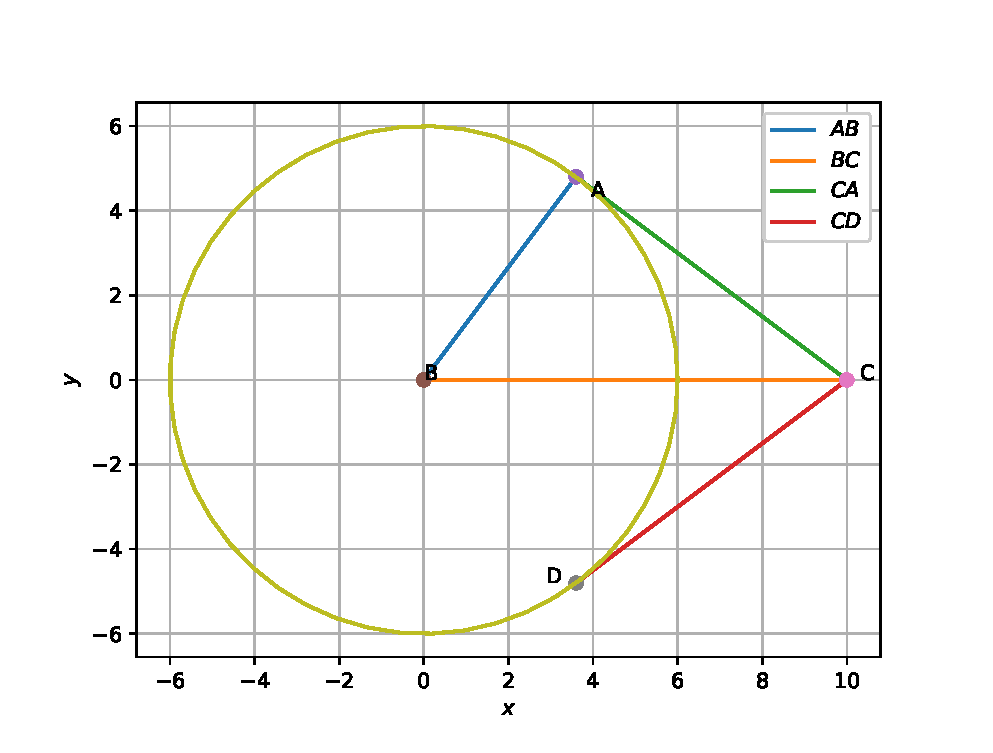
\includegraphics[width=\columnwidth]{./solutions/6/codes/circle/exercise/circle.eps}
\caption{}
\label{fig:4.2.6_circ_1}
\end{figure}

